%--------------------------------------
% Create title frame
\titleframe

%--------------------------------------
% Table of contents
%\begin{frame}{Overview}
%  \setbeamertemplate{section in toc}[sections numbered]
%  \tableofcontents[hideallsubsections]
%\end{frame}

\section{El concepto de `fractal'}

\begin{frame}{\insertsectionhead}
\framesubtitle{Estructuras que siguen patrones repetitivos}

\begin{figure}[ht!]
    \begin{subfigure}[b]{0.3\textwidth}
      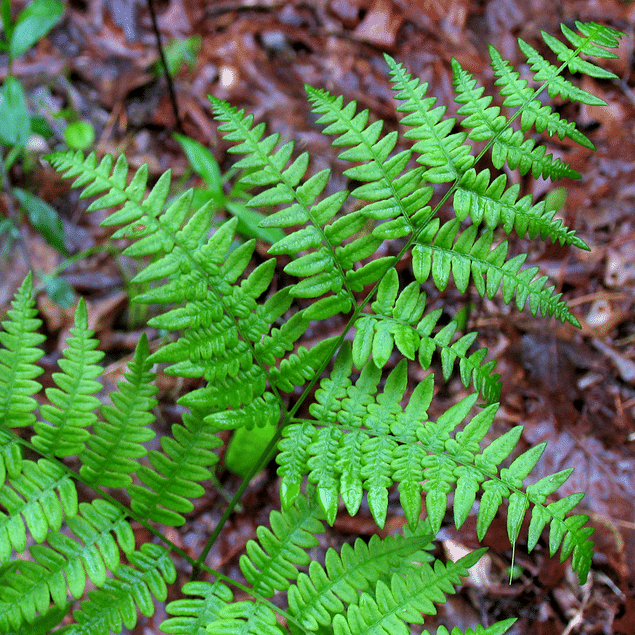
\includegraphics[width=\textwidth]{screenshots/helecho.png}
      \caption*{Helecho}
    \end{subfigure}
    \hspace{\fill}
    \begin{subfigure}[b]{0.3\textwidth}
      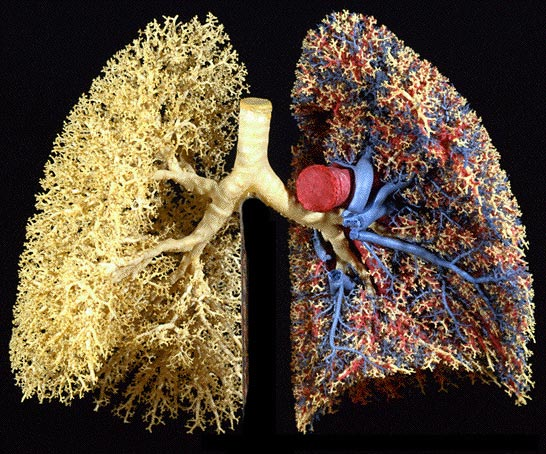
\includegraphics[width=\textwidth]{screenshots/lungs.jpg}
      \caption*{Pulmones}
    \end{subfigure}
    \hspace{\fill}
    \begin{subfigure}[b]{0.3\textwidth}
      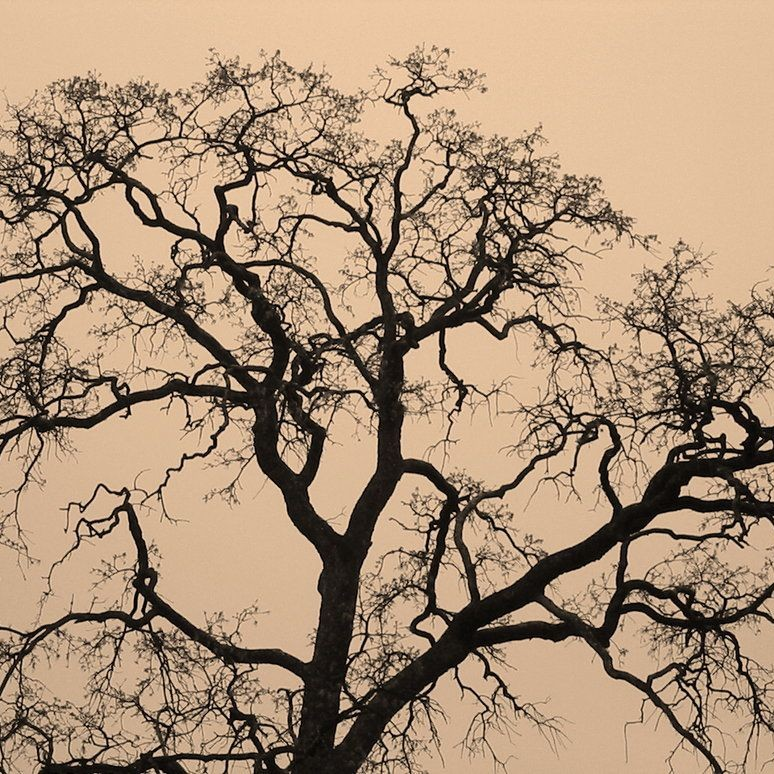
\includegraphics[width=\textwidth]{screenshots/tree.jpg}
      \caption*{Árbol}
    \end{subfigure}
  \end{figure}
  
  \pause
  \vspace{\fill}
  \centering {\Large \textbf{Autosimilaridad}}

    
\end{frame}

\begin{frame}{\insertsectionhead}
\framesubtitle{Fractales clásicos}

\begin{figure}[ht!]
    \begin{subfigure}[b]{0.3\textwidth}
      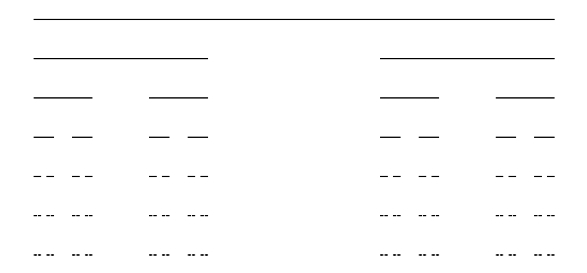
\includegraphics[width=\textwidth]{screenshots/Cantor.png}
      \caption*{Conjunto de Cantor}
    \end{subfigure}
    \hspace{\fill}
    \begin{subfigure}[b]{0.2\textwidth}
      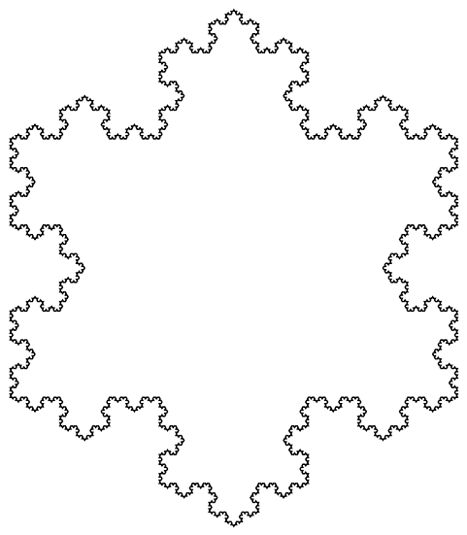
\includegraphics[width=\textwidth]{screenshots/Koch.png}
      \caption*{Copo de Koch}
    \end{subfigure}
    \hspace{\fill}
    \begin{subfigure}[b]{0.23\textwidth}
      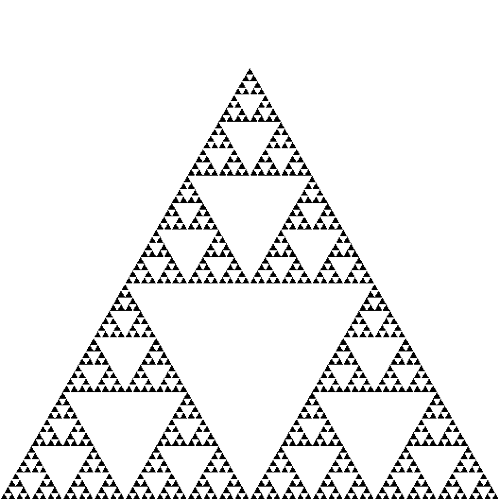
\includegraphics[width=\textwidth]{screenshots/Sierpinski.png}
      \caption*{Triángulo de Sierpinski}
    \end{subfigure}
     \hspace{\fill}
    \begin{subfigure}[b]{0.23\textwidth}
      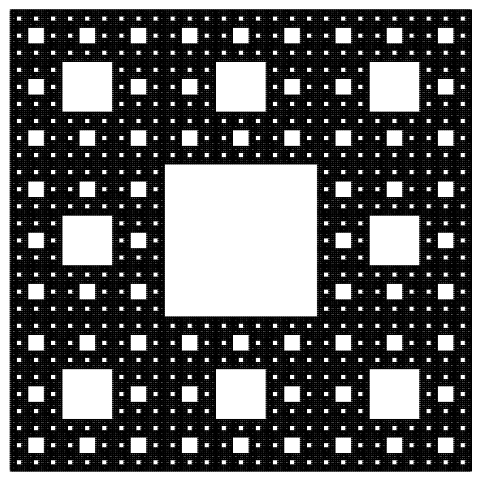
\includegraphics[width=\textwidth]{screenshots/alfombra.png}
      \caption*{Alfombra de Sierpinski}
    \end{subfigure}
  \end{figure}
\vspace{\fill}
\pause
\centering Autosimilares y su dimensión no es un número entero.

\end{frame}

\begin{frame}{\insertsectionhead}
  \framesubtitle{Definición de fractal según B. Mandelbrot}
  \begin{columns}[c, onlytextwidth]
    \column{0.47\textwidth}
        {\Large\textit{Un \textbf{fractal} es un subconjunto de $\mathbb R^n$ que es autosimilar y cuya dimensión fractal excede a su dimensión topológica.}}
        
        \begin{flushright}
        {\large\textit{Benoit Mandelbrot}}
        \end{flushright}
    \hfill
    \column{0.47\textwidth}
    \center
    \resizebox{0.5\textheight}{!}{%
      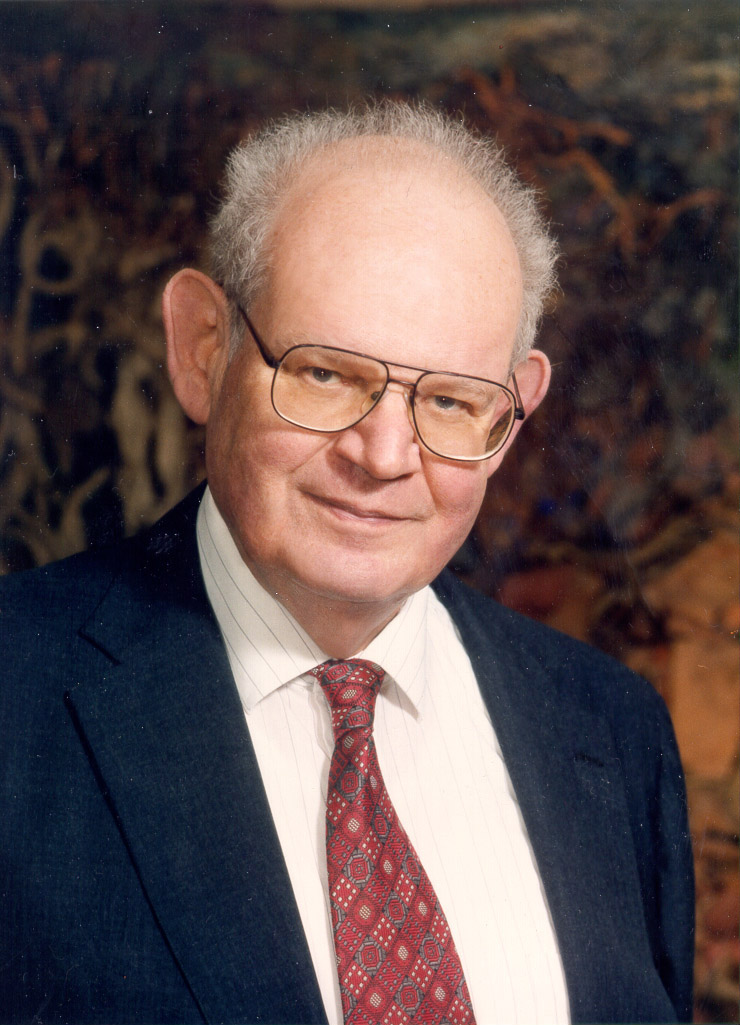
\includegraphics[]{screenshots/mandelbrot.jpg}
    }
  \end{columns}
\end{frame}

\section{Generación de fractales}

\begin{frame}{\insertsectionhead}

{\Large Existen distintas formas de generar fractales, pero todas se basan en la misma idea.}
\pause
\vfill
\centering
{\LARGE \textbf{La Iteración}}
\vspace{\fill}
\pause
\begin{itemize}
    \item {\Large Iteración de funciones complejas.}
    \item {\Large Iteración de aplicaciones contractivas (SFI).}
    \item {\Large Métodos iterativos de visualización (Sphere-Tracing).}
\end{itemize}
    
\end{frame}

\section{Iteración de funciones complejas}

\begin{frame}{\insertsectionhead}
    
{\large
Sean $f:\mathbb C\longrightarrow \mathbb C$ una función compleja y $z_0\in\mathbb C$. 
\pause

\textbf{Sucesión de iteradas:}
$$
\{f^n(z_0)\} = z_0, f(z_0), f(f(z_0)), \dots
$$
\pause
\textbf{Órbita de $z_0$:}
$$
O_f(z_0)=\{f^n(z_0) : n\in\mathbb N\}
$$
\pause
\begin{itemize}
    \item \textbf{Distintos comportamientos} de la sucesión de iteradas en cada $z_0\in\mathbb C$: convergente, divergente, cíclica o caótica.
    \item Dependiendo de dicho comportamiento \textbf{asignamos un color}.
\end{itemize}

}
\end{frame}

\begin{frame}{\insertsectionhead}
\framesubtitle{Teorema del punto fijo de Banach}
{\large 
\begin{block}{Teorema}
\begin{itemize}
    \item $X$ espacio métrico \textbf{completo}.
    \item $f:X\longrightarrow X$ una aplicación \textbf{contractiva}
\end{itemize}

Entonces

\begin{itemize}
    \item $f$ tiene un \textbf{único punto fijo} $x^*$.
    \item La \textbf{sucesión de iteradas} $\{f^n(x_0)\}$ converge a $x^*$ para cualquier $x_0\in X$ inicial.
\end{itemize}
\end{block}
\pause

\textbf{Aplicaciones del teorema del punto fijo}: Método de Newton y Sistemas de Funciones Iteradas.

}
\end{frame}

\begin{frame}{\insertsectionhead}
\framesubtitle{Método de Newton}

El \textbf{método de Newton} es un proceso iterativo utilizado para calcular raíces de una función $f:\mathbb C \longrightarrow\mathbb C$ a partir de un término $z_0\in\mathbb C$.

\begin{figure}[ht!]
\hspace{\fill}
    \begin{subfigure}[b]{0.3\textwidth}
      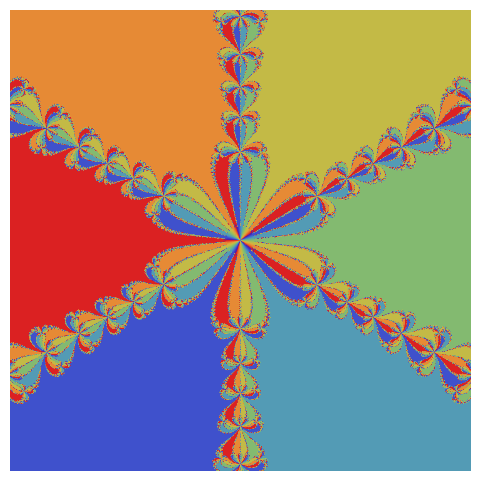
\includegraphics[width=\textwidth]{screenshots/cuencas-4.png}
      \caption*{Según la raíz a la que converge}
    \end{subfigure}
    \hspace{\fill}
    \begin{subfigure}[b]{0.3\textwidth}
      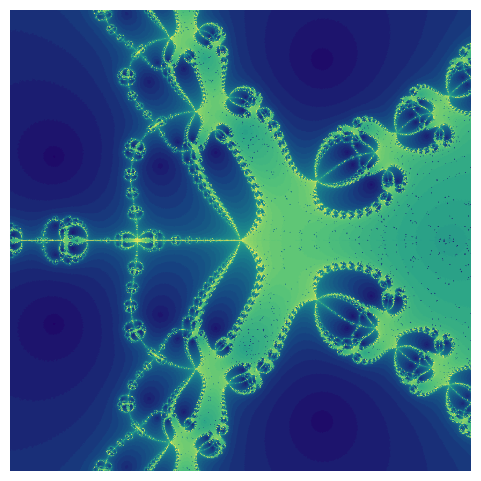
\includegraphics[width=\textwidth]{screenshots/newton-velocidad.png}
      \caption*{Según las iteraciones dadas}
    \end{subfigure}
    \hspace{\fill}
  \end{figure}

    
\end{frame}

\begin{frame}{\insertsectionhead}
\framesubtitle{Conjuntos de Julia}
{\large 
Presentamos la familia de funciones 

$$
P_c(z) = z^2 + c
$$ con $z,c\in\mathbb C$.
\vfill
Si fijamos una constante $c\in\mathbb C$ e iteramos $P_c(z_0)$ para cada $z_0\in\mathbb C$ obtenemos los llamados \textbf{Conjuntos de Julia} $\mathcal{J}_c$.
}
\end{frame}


\begin{frame}{\insertsectionhead}
\framesubtitle{Conjuntos de Julia}
    \begin{figure}[ht!]
\hspace{\fill}
    \begin{subfigure}[b]{0.3\textwidth}
      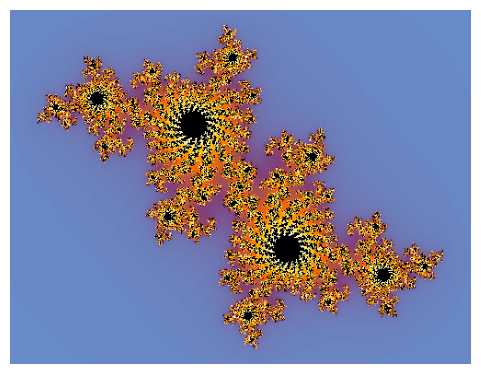
\includegraphics[height=4cm]{screenshots/Julia.png}
      \caption*{{\normalsize $\mathcal{J}_{-0.23+0.65i}$}}
    \end{subfigure}
    \hspace{\fill}
    \begin{subfigure}[b]{0.3\textwidth}
      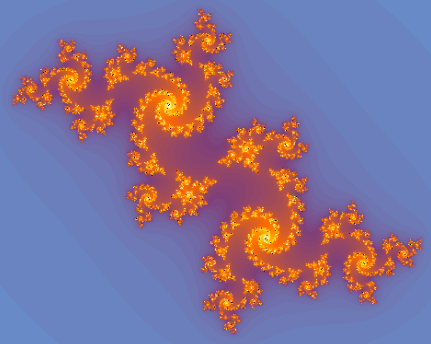
\includegraphics[height=4cm]{screenshots/juliaSetPlot-1.png}
      \caption*{{\normalsize $\mathcal{J}_{-0.23+0.69i}$}}
    \end{subfigure}
    \hspace{\fill}
  \end{figure}
  \centering  {\Large Por tanto, hay tantos conjuntos de Julia como números complejos.}

\end{frame}

    


\begin{frame}{\insertsectionhead}
\framesubtitle{Conjunto de Mandelbrot}

{\large 
Si fijamos una condición inicial $z_0=0$ e iteramos para cada posible valor de $c$ visualizaremos el \textbf{Conjunto de Mandelbrot} $\mathcal{M}$. }

\begin{figure}[ht!]
\hspace{\fill}
\begin{subfigure}[b]{0.3\textwidth}
  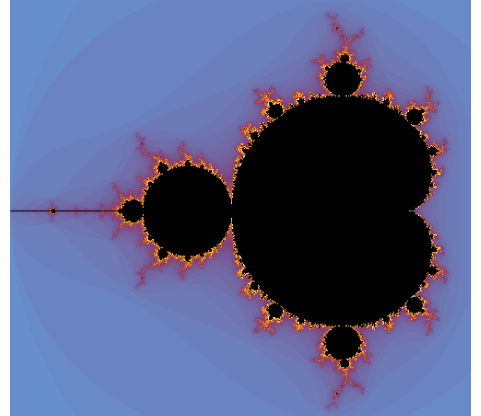
\includegraphics[width=\textwidth]{screenshots/Mandelbrot-Mathematica.png}
  \caption*{Conjunto de Mandelbrot}
\end{subfigure}
\hspace{\fill}
\begin{subfigure}[b]{0.3\textwidth}
  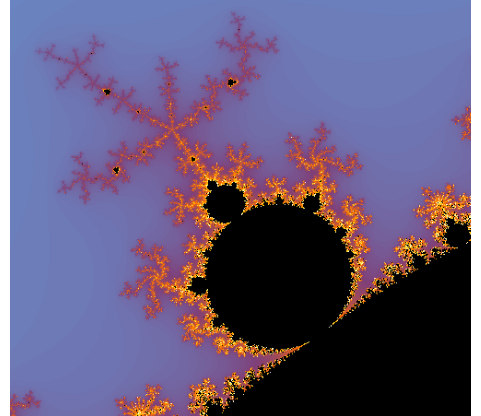
\includegraphics[width=\textwidth]{screenshots/MandelbrotSetPlot.png}
  \caption*{Detalle ampliado de $\mathcal{M}$}
\end{subfigure}
\hspace{\fill}
\end{figure}

\end{frame}

\section{Sistemas de Funciones Iteradas}

\begin{frame}{\insertsectionhead}
\framesubtitle{Definición}
{\large 
Un \textbf{Sistema de Funciones Iteradas (SFI)} está formado por:
\begin{itemize}
    \item Un espacio métrico completo $X$.
    \item Un conjunto finito de aplicaciones contractivas $\{w_1,\dots,w_n\}.$
\end{itemize}

Dado un conjunto compacto $A\subset X$, consideramos aplicación $W$ definida como

$$
W(A) = \bigcup_{i=1}^n w_i(A) 
$$

En particular, en $\mathbb R^2$ y mediante transformaciones afines contractivas podemos construir SFI.
}
\end{frame}

\begin{frame}{\insertsectionhead}
\framesubtitle{Convergencia de SFI}

{\large La iteración infinita de la aplicación $W$ finalmente converge a un \textbf{atractor}.}

\begin{figure}[ht!]
\hspace{\fill}
\begin{subfigure}[b]{0.4\textwidth}
  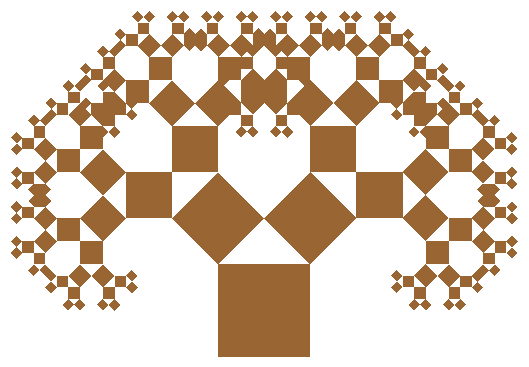
\includegraphics[height=4cm]{screenshots/arbol-pitagoras.png}
  \caption*{Árbol de Pitágoras}
\end{subfigure}
\hspace{\fill}
\begin{subfigure}[b]{0.2\textwidth}
  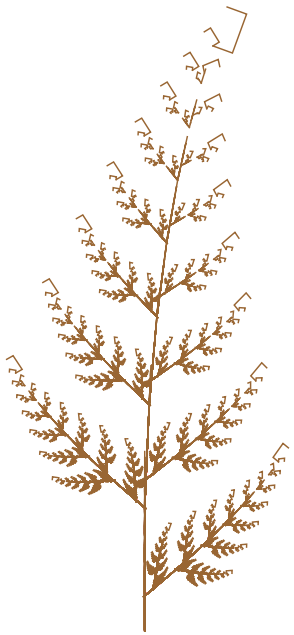
\includegraphics[height=4cm]{screenshots/helecho-barnsley.png}
  \caption*{Helecho de Barnsley}
\end{subfigure}
\hspace{\fill}
\end{figure}
    
\end{frame}

\begin{frame}{\insertsectionhead}
\framesubtitle{El problema inverso}
{\large
\centering Obtener imágenes a partir de SFI \checked

\centering ¿Obtener SFI a partir de imágenes? \pause Solución: \textbf{El teorema del Collage}.
}
\vspace{\fill}
\centering 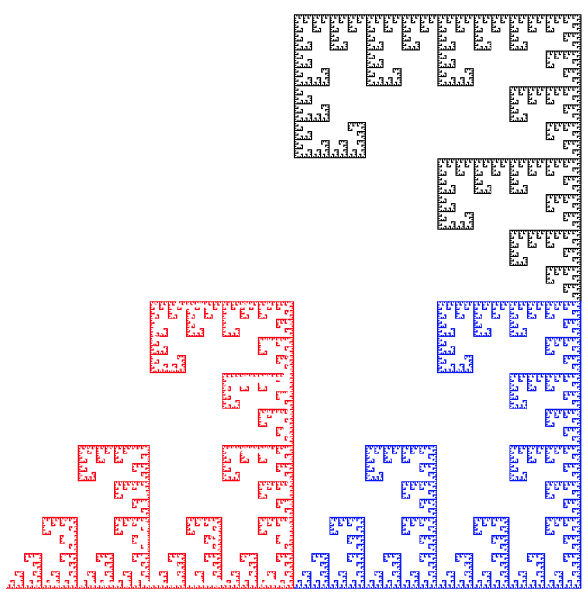
\includegraphics[width=4.5cm]{screenshots/collage.png}
    
\end{frame}

\section{Uso de WebGL}

\begin{frame}{\insertsectionhead}
\framesubtitle{GPU vs CPU}

\begin{figure}[ht!]
\hspace{\fill}
\begin{subfigure}[b]{0.3\textwidth}
  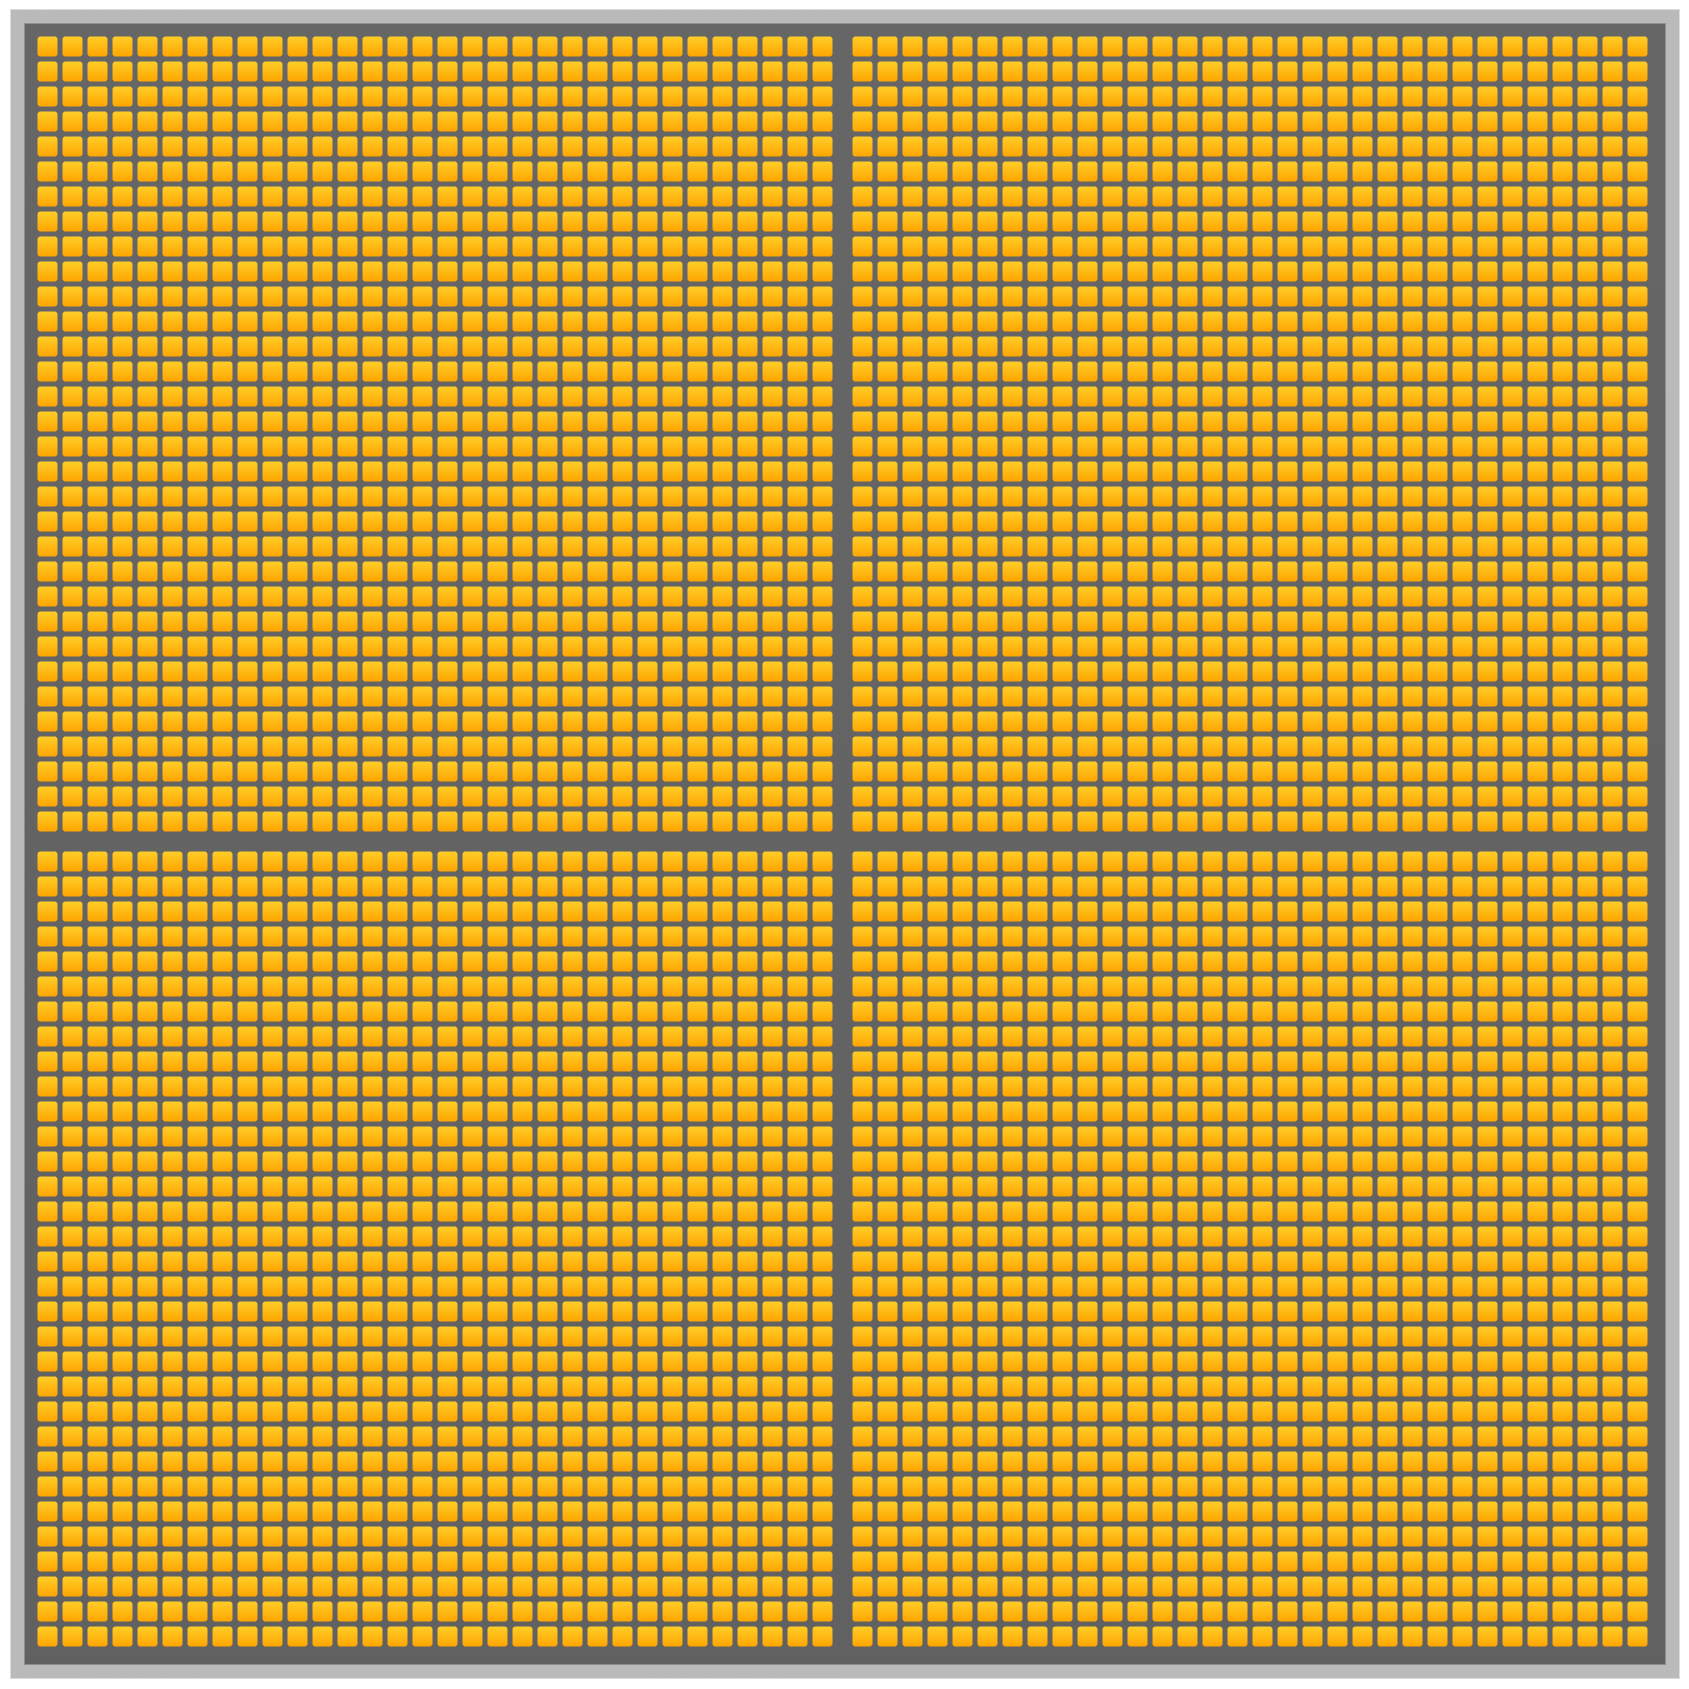
\includegraphics[width=\textwidth]{screenshots/GPU.drawio.png}
  \caption*{GPU}
\end{subfigure}
\hspace{\fill}
\begin{subfigure}[b]{0.3\textwidth}
  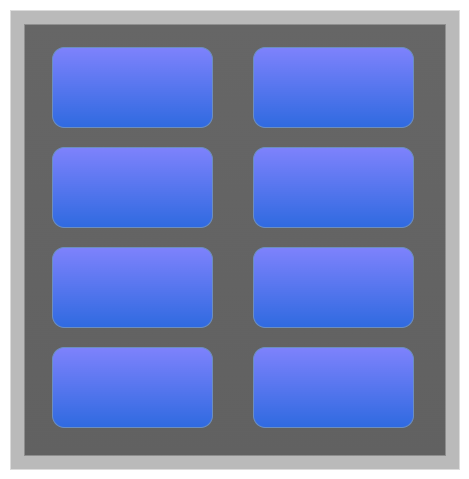
\includegraphics[width=\textwidth]{screenshots/CPU.drawio.png}
  \caption*{CPU}
\end{subfigure}
\hspace{\fill}
\end{figure}

\centering {\large WebGL utiliza CPU (JavaScript) y GPU (GLSL)}
    
\end{frame}

\section{Visualización de fractales 2D}
\begin{frame}{\insertsectionhead}
    \framesubtitle{Conjuntos de Julia y Mandelbrot}
    {\large
    Posibilidad de identificar la pantalla con el plano complejo:
    
    \pause
    
    \centering\textbf{Cada píxel es un número complejo}
    
    
    Transcribimos el algoritmo a código GLSL y el resultado es ...}
    
    \begin{figure}[ht!]
    \hspace{\fill}
    \begin{subfigure}[b]{0.4\textwidth}
      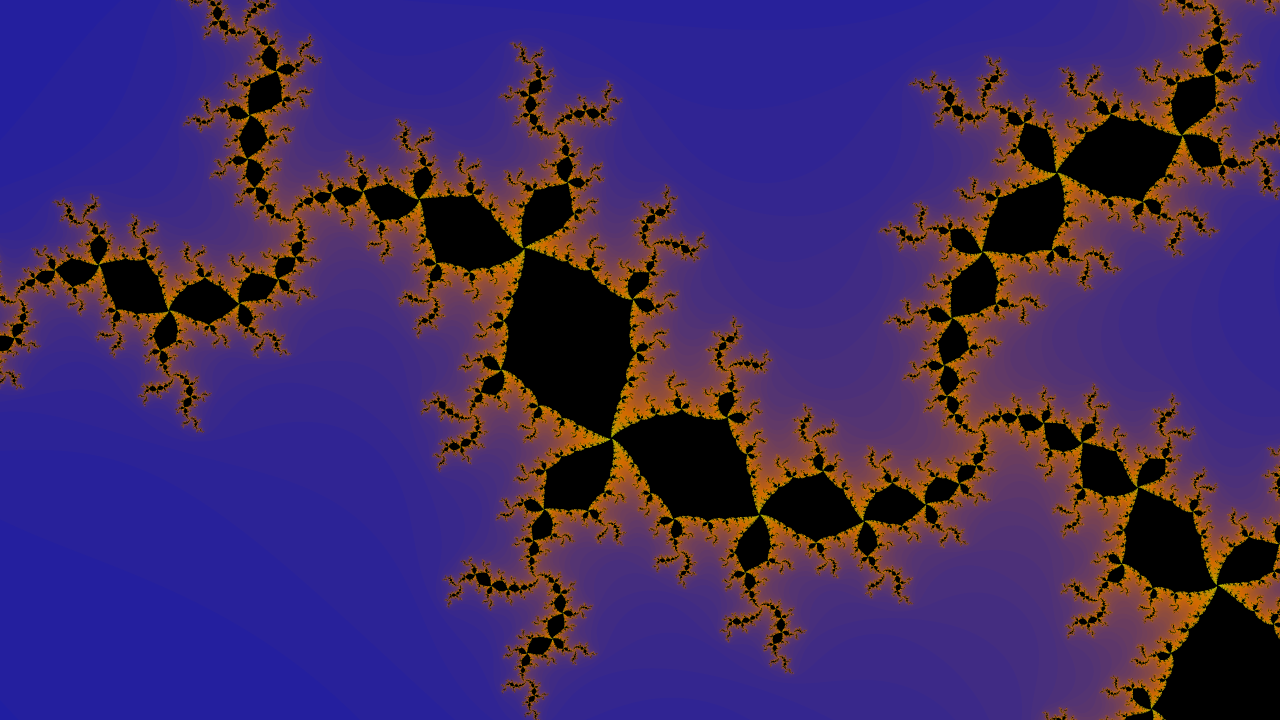
\includegraphics[width=\textwidth]{screenshots/julia-WEBGL.png}
    \end{subfigure}
    \hspace{\fill}
    \begin{subfigure}[b]{0.4\textwidth}
      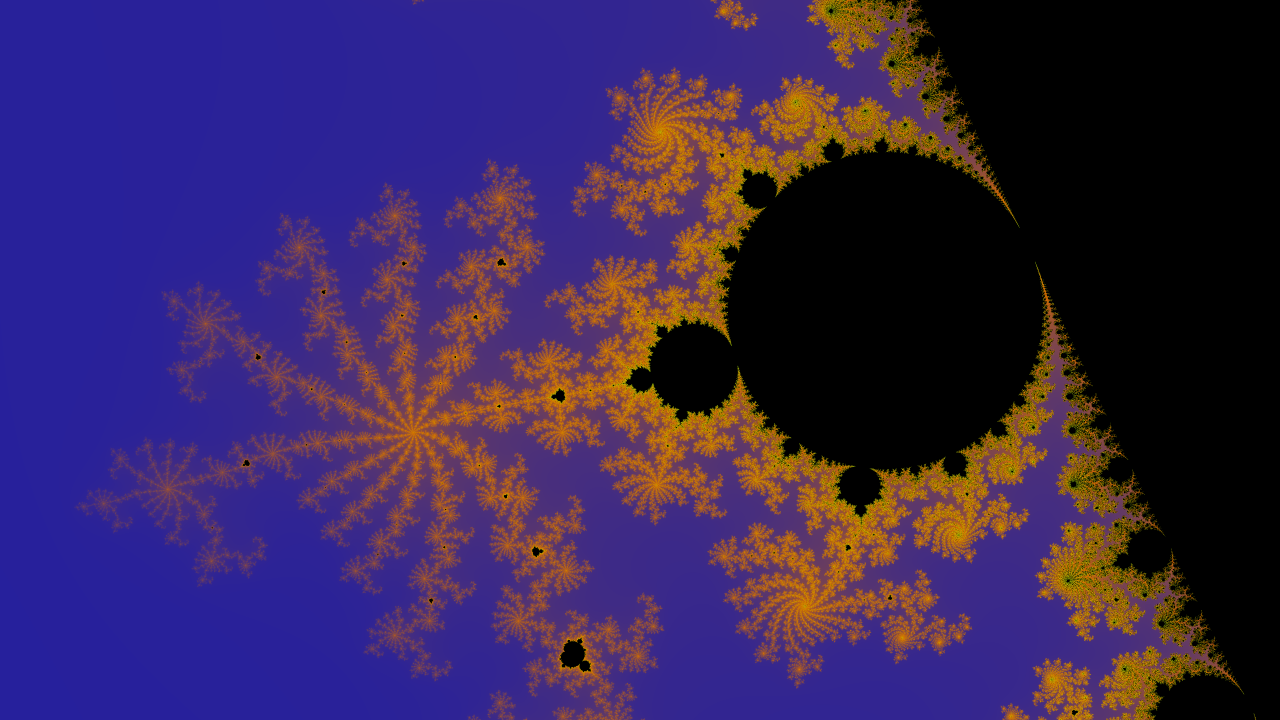
\includegraphics[width=\textwidth]{screenshots/mandelbrot-WEBGL.png}
    \end{subfigure}
    \hspace{\fill}
    \end{figure}
    
\end{frame}

\section{Ray-Tracing}
\begin{frame}{\insertsectionhead}
\framesubtitle{Fundamentos}
{\large 
\begin{itemize}
    \item \textbf{Rasterización}: Identificar qué píxeles ocupan los objetos de la escena.
    \item \textbf{Ray-Tracing}: Identificar qué objeto se proyectan sobre cada píxel.
\end{itemize}

\pause

\begin{columns}[c, onlytextwidth]
    \column{0.45\textwidth}
        
        Componentes de un programa `ray-tracer':
        
        \begin{itemize}
            \item Generación de rayos primarios
            \item Cálculo de intersecciones
            \item Modelo de iluminación local
        \end{itemize}
        
    \hfill
    \column{0.52\textwidth}
    \center
    \resizebox{0.9\textheight}{!}{%
      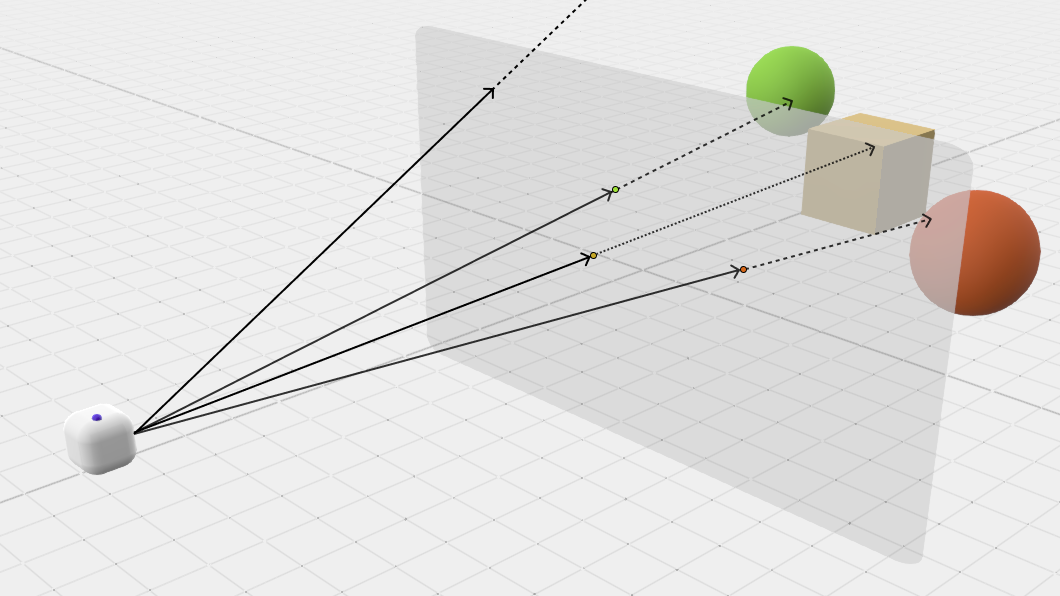
\includegraphics[]{screenshots/RT.png}
    }
  \end{columns}
}

\end{frame}

\begin{frame}{\insertsectionhead}

\centering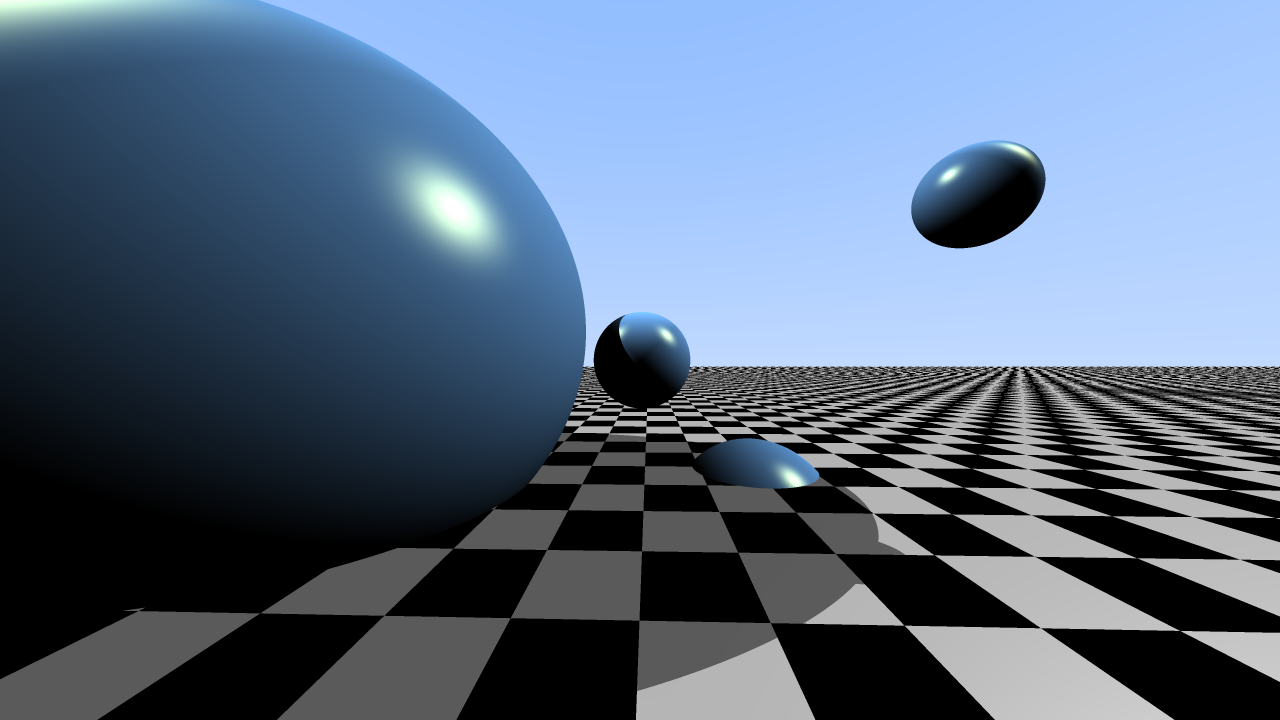
\includegraphics[width=11cm]{screenshots/imagen-final.png}
    
\end{frame}

\section{Visualización de fractales 3D}

\begin{frame}{\insertsectionhead}
\framesubtitle{Sphere-Tracing}
{\large

Es sencillo calcular la intersecciones rayo-esfera y rayo-plano, pero

\centering\textbf{¿Cómo calculamos la intersección con un fractal?}

\centering Solución: Con el algoritmo \textbf{Sphere-Tracing}.

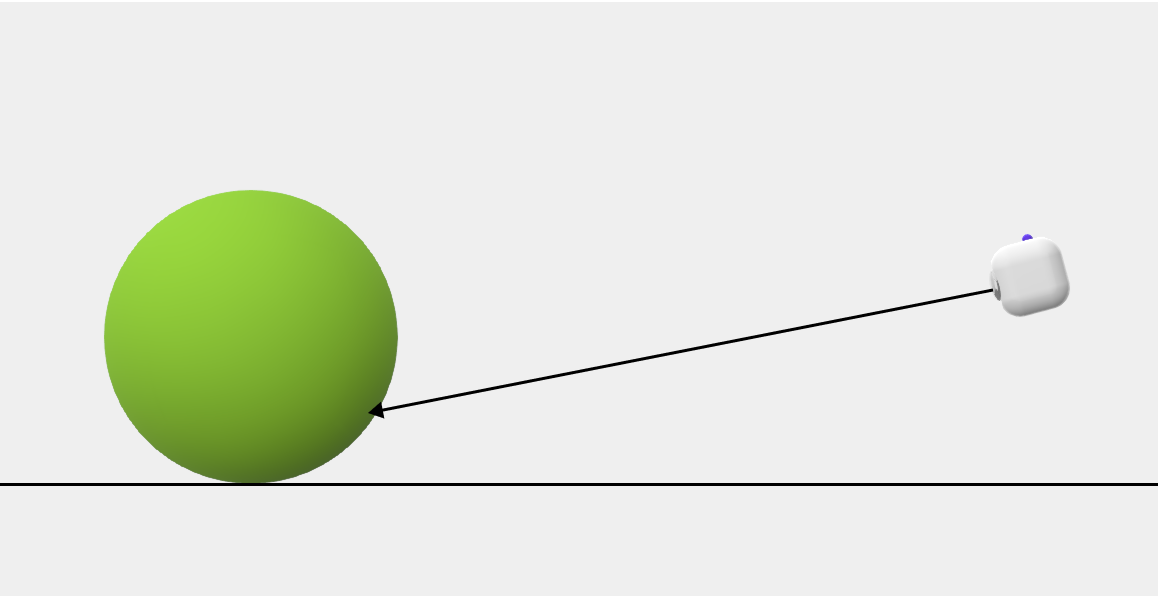
\includegraphics[width=8.5cm]{screenshots/ST-1.png}

}
    
\end{frame}

\begin{frame}{\insertsectionhead}
\framesubtitle{Sphere-Tracing}

\centering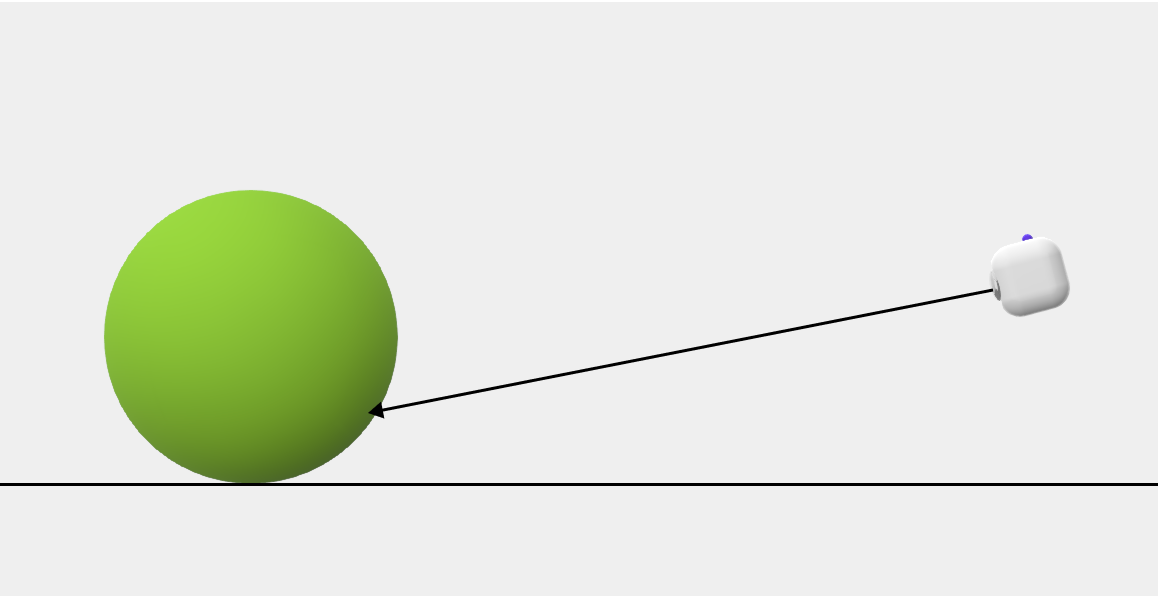
\includegraphics[width=11cm]{screenshots/ST-1.png}
    
\end{frame}

\begin{frame}{\insertsectionhead}
\framesubtitle{Sphere-Tracing}

\centering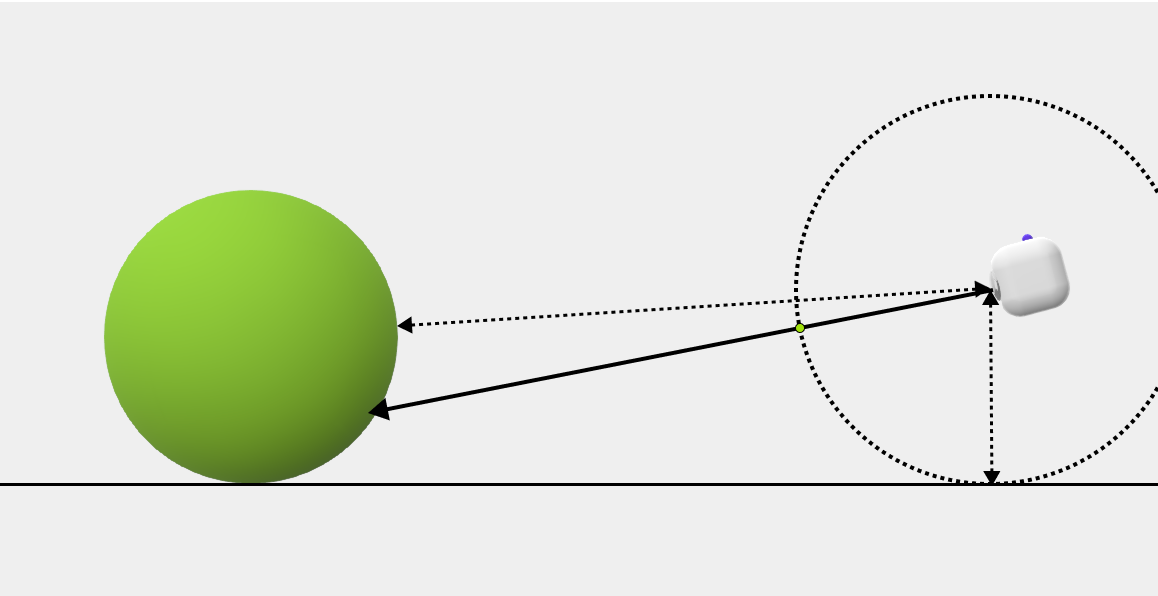
\includegraphics[width=11cm]{screenshots/ST-2.png}
    
\end{frame}

\begin{frame}{\insertsectionhead}
\framesubtitle{Sphere-Tracing}

\centering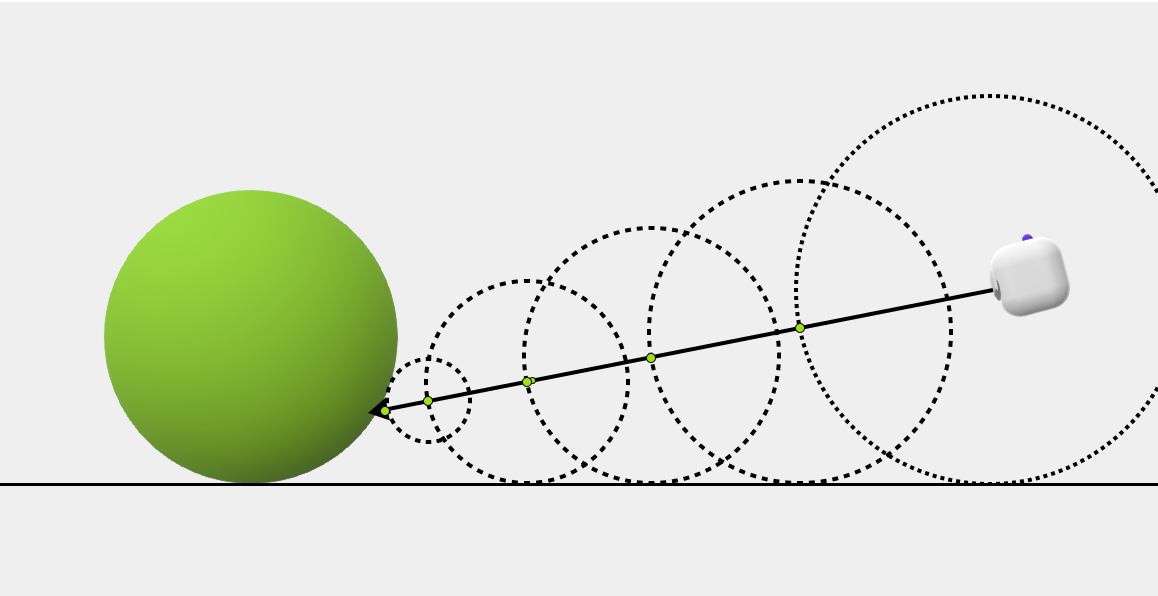
\includegraphics[width=11cm]{screenshots/ST-3.png}
    
\end{frame}

\begin{frame}{\insertsectionhead}
\framesubtitle{Sphere-Tracing}

\centering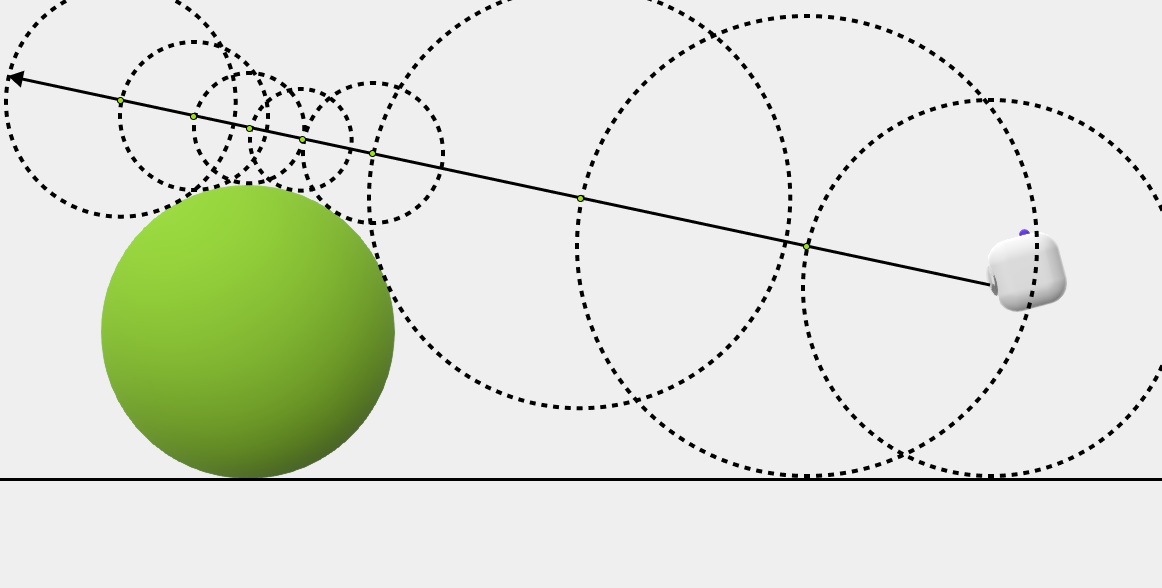
\includegraphics[width=11cm]{screenshots/ST-Miss.png}
    
\end{frame}

\begin{frame}{\insertsectionhead}
\framesubtitle{BDFs y SDFs}
{\large 
Necesitamos estimar la distancia de un punto cualquiera al fractal... o al menos una cota inferior.

\pause

Para ello contamos con las \textbf{BDF} (Bounding Distance Function), que son funciones $f:\mathbb R^3\longrightarrow \mathbb R$ tales que

$$
|f(x)|\leq d(x,f^{-1}(0)) \ \ \forall x\in\mathbb R^3
$$

Es decir, acotan la distancia a la superficie implícita que definen.

Si se cumple la igualdad, entonces se les denomina \textbf{SDF} (Signed Distance Function).
}
\end{frame}

\begin{frame}{\insertsectionhead}
\framesubtitle{Conjuntos de Julia y Mandelbrot 3D}
{\large 
Generalización de los complejos $\mathbb C$: los \textbf{cuaternios} $\mathbb H$.

%\vspace{\fill} 
\pause

Podemos extender la función $P_c(z)=z^2+c$ a 

$$
P(q) = q^2 + c,\text{ con }q,c\in\mathbb H
$$

}

    \begin{figure}[ht!]
    \hspace{\fill}
    \begin{subfigure}[b]{0.4\textwidth}
      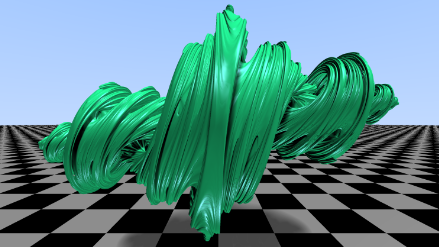
\includegraphics[width=\textwidth]{screenshots/julia-3D-frontal-2.png}
      \caption*{$\mathcal{J}_{-0.71-0.31i}$}
    \end{subfigure}
    \hspace{\fill}
    \begin{subfigure}[b]{0.4\textwidth}
      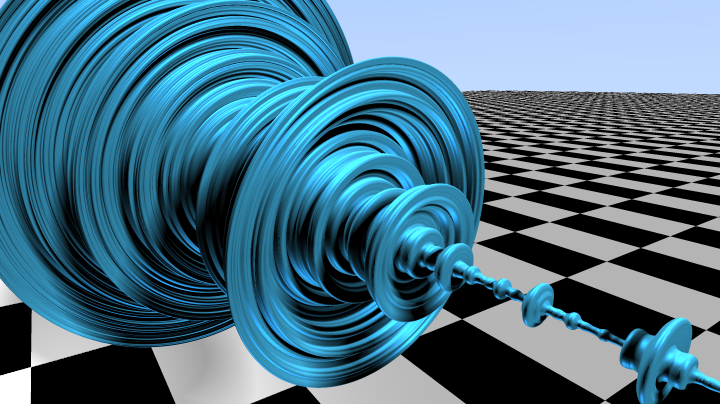
\includegraphics[width=\textwidth]{screenshots/mandelbrot-1.png}
      \caption*{$\mathcal{M}$ generalizado}
    \end{subfigure}
    \hspace{\fill}
    \end{figure}
\end{frame}

\begin{frame}{\insertsectionhead}
\framesubtitle{Conjunto de Mandelbub}

{\large Generalización de $\mathcal{M}_8$ (el conjunto de Mandelbrot utilizando la función $z^8+c$) utilizando aritmética poco rigurosa.

    \begin{figure}[ht!]
    \hspace{\fill}
    \begin{subfigure}[b]{0.4\textwidth}
      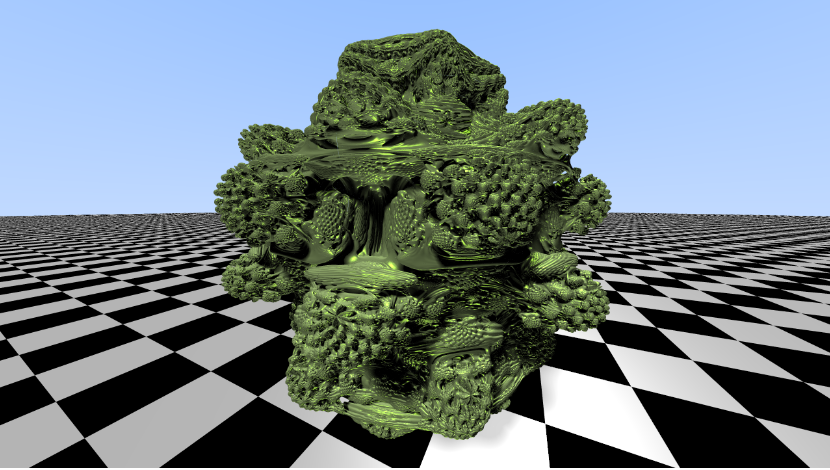
\includegraphics[width=\textwidth]{screenshots/mandelbub-1.png}
    \end{subfigure}
    \hspace{\fill}
    \begin{subfigure}[b]{0.4\textwidth}
      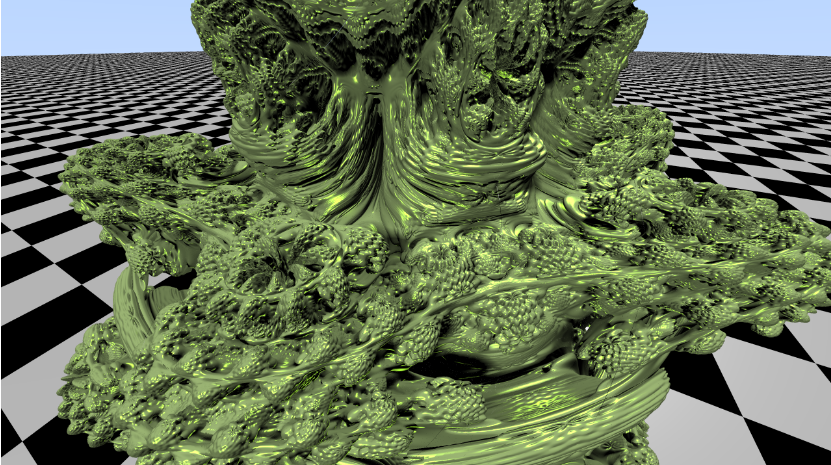
\includegraphics[width=\textwidth]{screenshots/mandelbub-2.png}
    \end{subfigure}
    \hspace{\fill}
    \end{figure}

}
    
\end{frame}

\section{Conclusión}

\begin{frame}{\insertsectionhead}

{\large 

La geometría fractal tiene aplicaciones en:
\begin{itemize}
    \item Desarrollo de videojuegos y producción de películas
    \item En otras áreas de las matemáticas como la estimación de parámetros mediante ecuaciones diferenciales e integrales
    \item Dinámica de poblaciones
    \item Procesos biológicos
    \item \dots
\end{itemize}
\vspace{\fill}

Diferencia entre la generación de imágenes en CPU y el uso de la GPU.

\vspace{\fill}
El siguiente paso sería optimizar la aplicación para que pudiera ejecutarse en tiempo real en ordenadores más convencionales.

}  
\end{frame}

\begin{frame}[allowframebreaks]{Bibliografía fundamental}

\begin{thebibliography}{99}

\bibitem{rubiano} Rubiano, G.N. (2013). \textit{Iteración y Fractales (con Mathematica ®)}. Universidad Nacional de Colombia.

\bibitem{Mandelbrot} Mandelbrot, B. (1983). \textit{The Fractal geometry of nature}. Freeman, New York.

\bibitem{Barnsley} Barnsley, M (1993). \textit{Fractals everywhere}. Academic Press, 2nd edition.

\bibitem{Shirley} Shirley, P. (2020). \textit{Ray Tracing in One Weekend}. Recuperado 28 de mayo de 2022, de \url{https://raytracing.github.io/books/RayTracingInOneWeekend.html}.

\bibitem{Hart-1989} Hart, J., Sandin, D. y Kauffman, L. (1989). Ray tracing deterministic 3-D fractals. \textit{ACM SIGGRAPH Computer Graphics}, 23(3):289--296. Disponible en \url{https://doi.org/10.1145/74334.74363}.

\bibitem{Hart-1995} Hart, J. (1995). Sphere Tracing: A Geometric Method for the Antialiased Ray Tracing of Implicit Surfaces. \textit{The Visual Computer}, 12:527--545. Disponible en \url{https://doi.org/10.1007/s003710050084}.

\bibitem{keenan-crane} Crane, K. (2005). Ray Tracing Quaternion Julia Sets on the GPU. \textit{University of Illinois at Urbana-Champaign}. Disponible en \url{https://www.cs.cmu.edu/~kmcrane/Projects/QuaternionJulia/paper.pdf}.

\bibitem{Hubbard-Douady} Douady, A. y Hubbard, J. (2009). \textit{Exploring the Mandelbrot set. The Orsay Notes}. Cornell University, Ithaca, NY. Disponible en \url{https://pi.math.cornell.edu/~hubbard/OrsayEnglish.pdf}.


\end{thebibliography}

\end{frame}

\begin{frame}{}


\vspace{1cm}

\centering\textbf{{\Huge ¡Gracias por escuchar!}}

\vspace{\fill}

 \begin{columns}[c, onlytextwidth]
    \column{0.47\textwidth}
        \vspace{0.7cm}
        \begin{center}
        
            \frame{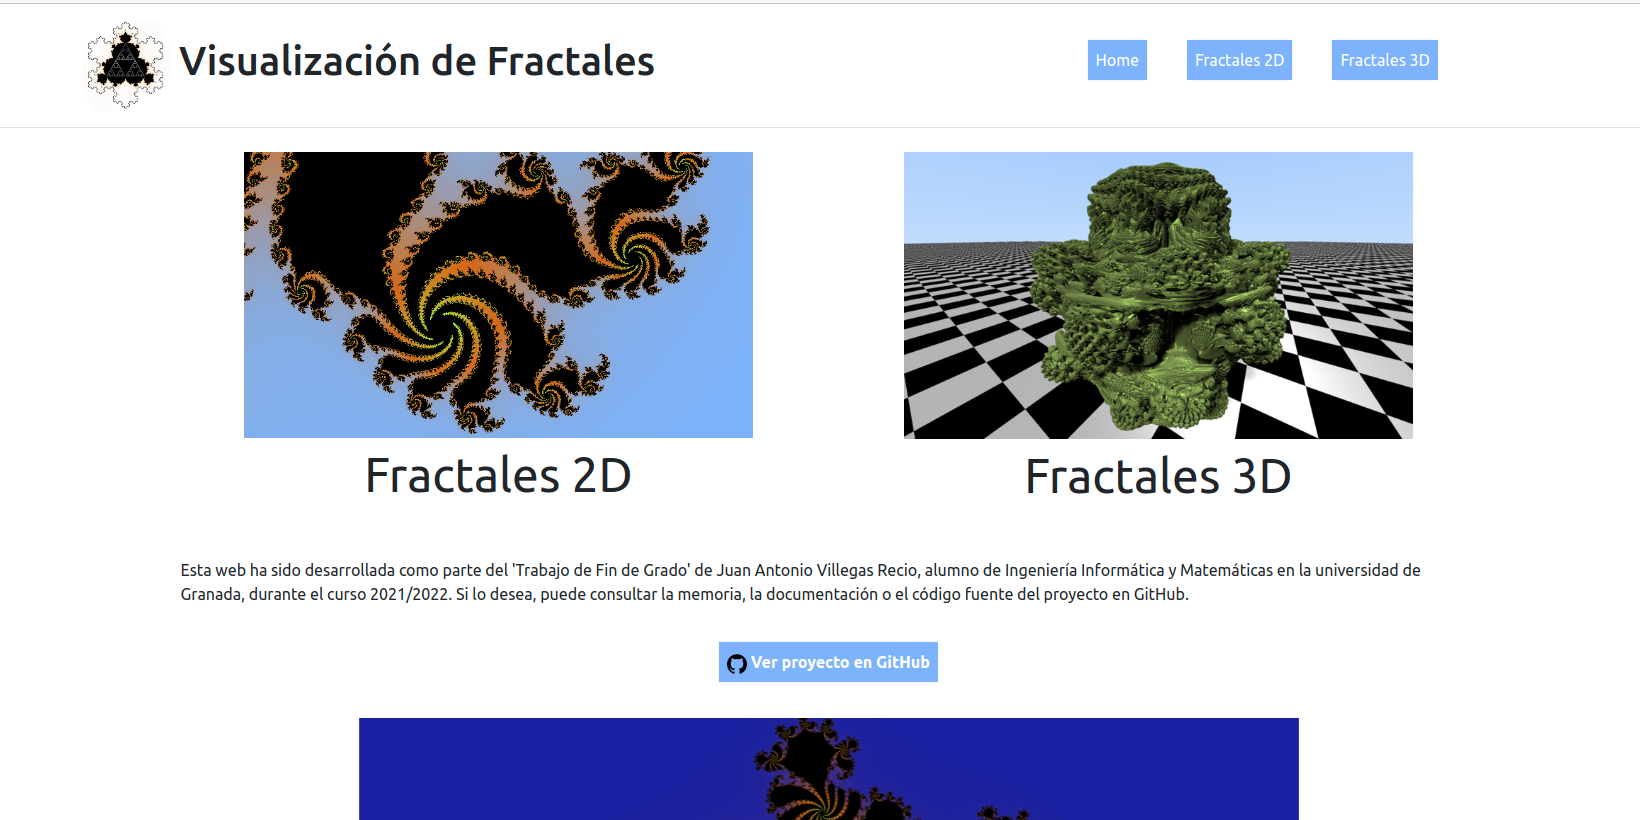
\includegraphics[width=\textwidth]{screenshots/enlace-web.png}}       
            
            Web disponible en  
            
            \url{jantoniovr.github.io/Geometria-Fractal/}
            
        \end{center}
        
        
    \hfill
    \column{0.47\textwidth}
        \begin{center}
            
            
            \frame{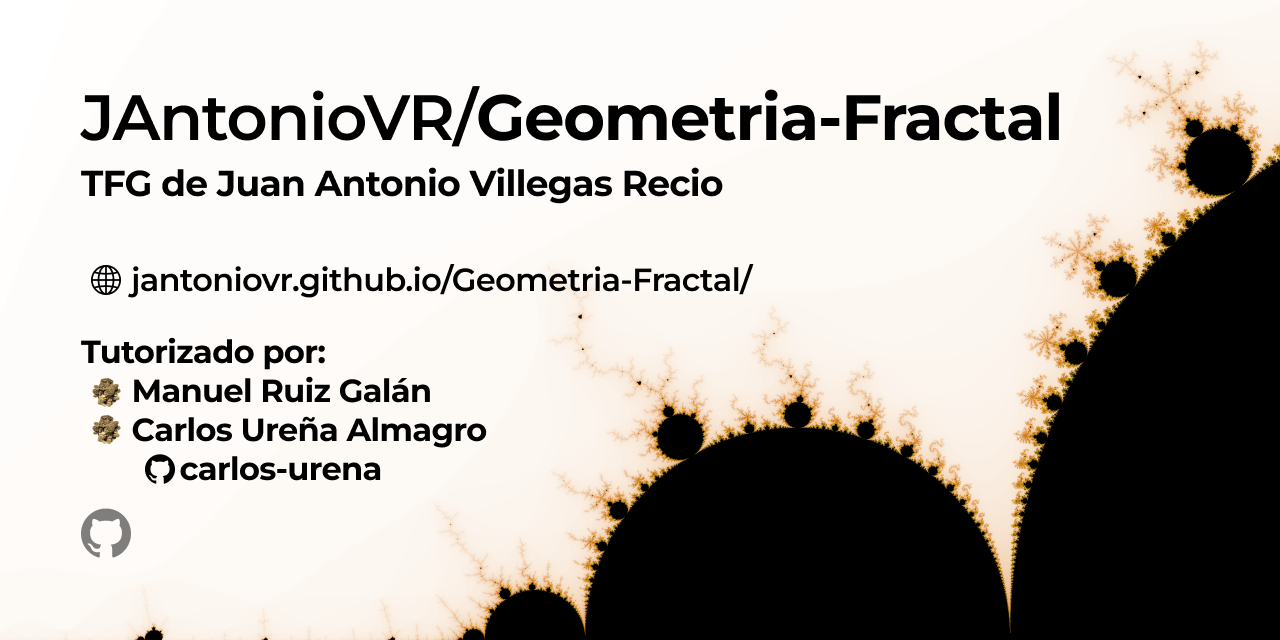
\includegraphics[width=\textwidth]{screenshots/portada-repo-final.png}}
            
            Repositorio de GitHub disponible en 
            
            \url{github.com/JAntonioVR/Geometria-Fractal}
            
        \end{center}
        
  \end{columns}

    
\end{frame}